% In the background chapter you should provide all the information required to acquire a sufficient knowledge to understand other chapters of the report. Suppose the reader is not familiar with the topic; so, for instance, if your project was focused on implementing a VPN, explain what it is and how it works. This chapter is supposed to work kind of like a "State of the Art" chapter of a thesis.\\ Organize the chapter in multiple sections and subsections depending on how much background information you want to include. It does not make any sense to mix background information about several topics, so you can split the topics in multple sections.\\Assume that the reader does not know anything about the topics and the tecnologies, so include in this chapter all the relevant information. Despite this, we are not asking you to write 20 pages in this chapter. Half a page, a page, or 2 pages (if you have a lot of information) for each `topic`(i.e. FreeRTOS, the SEcube, VPNs, Cryptomator, PUFs, Threat Monitoring....thinking about some of the projects...).
\chapter{Background}
In this era, as technology has become an integral part of modern life, digital security has become crucial. Hardware security is becoming even more significant, along with the need for development and research of robust hardware security measures.
As technology advances, so do cyber threats. The rise of IoT and interconnected devices is also a crucial factor.
In this environment, Physically Unclonable Functions (PUFs) have emerged as a promising approach to address the challenges of hardware authentication, secure key generation, and anti-counterfeiting measures. Among the various PUF implementations, Complementary Metal-Oxide-Semiconductor Arbiter PUFs (CAMPUFs) stand out as a powerful hardware security primitive based on CMOS technology.
\\
CAMPUFs leverage the unique physical variations inherent in CMOS integrated circuits to generate unpredictable and practically unclonable responses. The foundation of CMOS technology, with its low power consumption and high integration capabilities, makes it an ideal platform for building complex digital circuits and implementing PUFs.
\\
This chapter will provide an overview of the concepts that are the basis for the CamPUF design and that are needed in order to understand it.

\section{Physically Unclonable Functions}
A Physically Unclonable Function (PUF) is a security metric in hardware sistems based on inherent device physical variations to produce an unclonable, 
unique device response to a given input. Unclonability means that each PUF has a unpredictable response to a given input, due to the response being created by complex interactions between many random components.
The response acts as a unique device identifier, a sort of "digital fingerprint" for the device.

\subsection{Purposes} 
\begin{itemize}
\item \textbf{Key Generation}: PUFs can generate cryptographic keys directly from the unique physical responses of the ICs. These keys can be used for secure communication, encryption, and data protection.
\item \textbf{Challenge-Response Mechanism}: PUFs operate on a challenge-response mechanism, where a unique challenge is provided to the device, and the corresponding response is generated based on the unique physical characteristics of that particular IC.
\item \textbf{Randomness and Entropy Generation}: PUFs can serve as a high-quality source of randomness and entropy, critical for cryptographic protocols and secure communication.
\item \textbf{Authentication}: PUF responses can be used for secure device authentication, verifying the identity and integrity of hardware components in various applications, such as secure booting and secure firmware updates.
\item \textbf{Uniqueness and Unpredictability}: PUFs generate device-specific responses based on the inherent physical variations during manufacturing. As a result, each instance of the IC exhibits a unique response, making it practically impossible to clone or replicate the device.
\item \textbf{Anti-Counterfeiting Measures}: PUFs play a crucial role in preventing counterfeiting and unauthorized duplication of hardware components, as the uniqueness of the responses ensures the authenticity of genuine devices.
\end{itemize}

\subsection{Security Properties and Applications of PUFs}
\textbf{Key Security Properties of PUFs}
\begin{itemize}
\item \textbf{Unpredictability}: The inherent randomness linked to  PUF responses, even when given the same challenge multiple times. This property makes stonger the security of PUF-based authentication and key generation.
\item \textbf{Uniqueness and Unclonability}: PUFs depend on the uniqueness of their physical microstructure. This microstructure depends on random physical factors introduced during manufacturing that gives unique reponses. These factors are unpredictable and uncontrollable, which makes it virtually impossible to duplicate or clone the structure.
\item \textbf{Resistance to Physical Attacks}: PUFs are resilient against various physical attacks, including invasive attacks like reverse engineering and probing, as well as non-invasive attacks like side-channel analysis.
\end{itemize}
\textbf{Practical Applications of PUFs}
\begin{itemize}
\item \textbf{Secure Key Generation}: PUF responses can be utilized to generate cryptographic keys without the need for additional storage of secret keys, enhancing the security of cryptographic protocols.This applciation is divided in Secret Key Distribution and Secret Key Storage.
\item \textbf{Hardware Authentication}: PUFs can be employed for secure device authentication, ensuring the legitimacy of hardware components and protecting against unauthorized access.
\item \textbf{Anti-Counterfeiting Measures}: PUFs serve as a powerful tool for detecting counterfeit devices, as the unique responses enable the verification of genuine products.
\item \textbf{Secure Communication}: PUF-based keys are valuable for securing communication channels, enabling secure and authenticated data transmission.
\end{itemize}

\subsection{Categories of Implementation}
PUFs can be categorized based on different operational principles and sources of randomness
\subsubsection{Intrinsic PUFs}

Intrinsic PUFs are characterized by their reliance on the inherent physical variations present within a single chip during the semiconductor manufacturing process. These variations arise due to manufacturing imperfections, process fluctuations, and random dopant fluctuations. The unique characteristics of each individual chip create a fingerprint-like response, making Intrinsic PUFs ideal for hardware authentication and identification purposes.
\\
Common Implementations of Intrinsic PUFs are:
\begin{itemize}
\item Delay PUFs: Delay PUFs exploit the differences in signal propagation delay along various paths within the circuit. By measuring these delays, a set of unique challenge-response pairs can be generated, forming the basis for secure authentication.
\item Ring Oscillator PUFs: Ring oscillator PUFs use the frequency differences in ring oscillators, circuits comprising an odd number of inverters. The varying delays in these oscillators result in distinctive response patterns, enabling the generation of cryptographic keys and unique device identifiers.
\item SRAM PUFs: SRAM PUFs exploit the randomness in the power-up behavior of standard static random-access memory on a chip as a PUF.
\item VIA PUFs: the Via PUFs technologies are based on "via" or "contact" formation during the standard CMOS fabrication process. 
\end{itemize}
\subsubsection{Extrinsic PUFs}

Extrinsic PUFs differ from Intrinsic PUFs as they derive their responses from external environmental factors that influence the behavior of the chip. These external factors may include temperature variations, light levels, power supply fluctuations, and electromagnetic interference. The responses generated by Extrinsic PUFs can change under different operating conditions, leading to additional sources of randomness.
\\
Common Implementations of Extrinsic PUFs are:
\begin{itemize}
\item Ambient Light PUFs: Ambient light PUFs utilize the incident light level on the chip's surface to create distinct response patterns. Variations in light intensity cause corresponding variations in the generated responses, enabling unique identification.
\item Temperature PUFs: Temperature PUFs exploit temperature-induced changes in the electrical characteristics of the chip. Different temperature levels result in varied responses, contributing to the unclonable behavior of the device.
\end{itemize}

\section{Fixed Pattern Noise}
Noise on digital cameras has a lot of sources, but two main categories can be identified
\begin{enumerate}
\item \textbf{Random Noise}: Not constant from frame to frame and can be reduced using frame averaging. In digital images, \textit{temporal noise} is often observed. It is
    completely random and results from variations in generating a value for a single pixel, converting photons into electrons. It is related to \textit{photon shot noise}, which depends on the number of photons
    that hit a single pixel during a prolonged exposure.
\item \textbf{Fixed Pattern Noise}: Caused by small differences in sensors pixels, often noticeable during long exposure shots. These small differences
    can be caused by variations in pixel size, or interferences in the sensor circuitry. External factors (such as temperature or exposure times) can also affect this type of noise.
    \\CMOS-based imaging devices are primarily affected by pattern noise. This is due to amplifiers present in the pixel columns and in all the CMOS sensor, introducing additional noise.
\end{enumerate}

\begin{figure}[h!]                      % REMEMBER TO REFERENCE THE IMAGE SOURCE
    \centering
    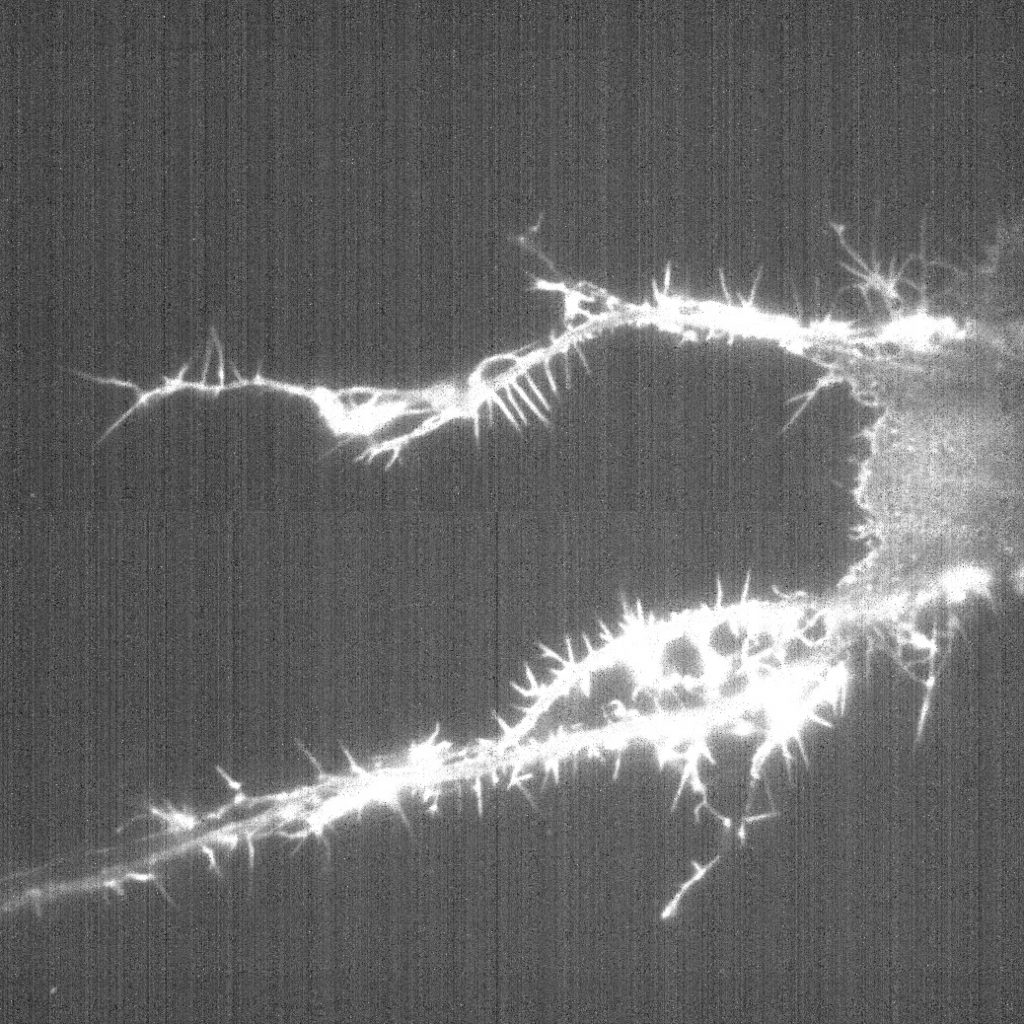
\includegraphics[width=0.6\textwidth]{images/Fixed_Noise_Pattern.jpeg}
    \caption{CMOS camera capting neurons. Average of 100 frames with 30ms exposure time.}
    \label{fig:fixedpatternnoise}
\end{figure}

Fixed Pattern Noise comes from two main sources: \textit{PRNU} (Photo Response Non-Uniformity) and \textit{DSNU} (Dark Signal Non-Uniformity).
Figure \ref{fig:fixedpatternnoise} shows fixed pattern noise on the background, the column patterns are present all over the image. Frame averaging usually works to eliminate random noise, but it worsen fixed pattern noise.

PRNU is caused by responsitivity variation between pixels and it is the dominant noise in illuminated images. PRNU has a lot of properties that make it useful as an image fingerprint.
It survives lossy JPEG compression and for this reason it has been used for source identification or forgery detection. This property, however, makes PRNU bad as the basis of a PUF.
Since it survives JPEG compression, the PRNU fingerprint can be obtained by anyone, if the image is shared without proper access control (an example would be an image shared on social media).

To address this security problem, the PUF design uses DSNU fingerprint as its basis. DSNU is more difficult to be extracted in illuminated natural images, since it is not the dominant noise.

\subsection{DSNU}
\begin{figure}[h!]                      % REMEMBER TO REFERENCE THE IMAGE SOURCE
    \centering
    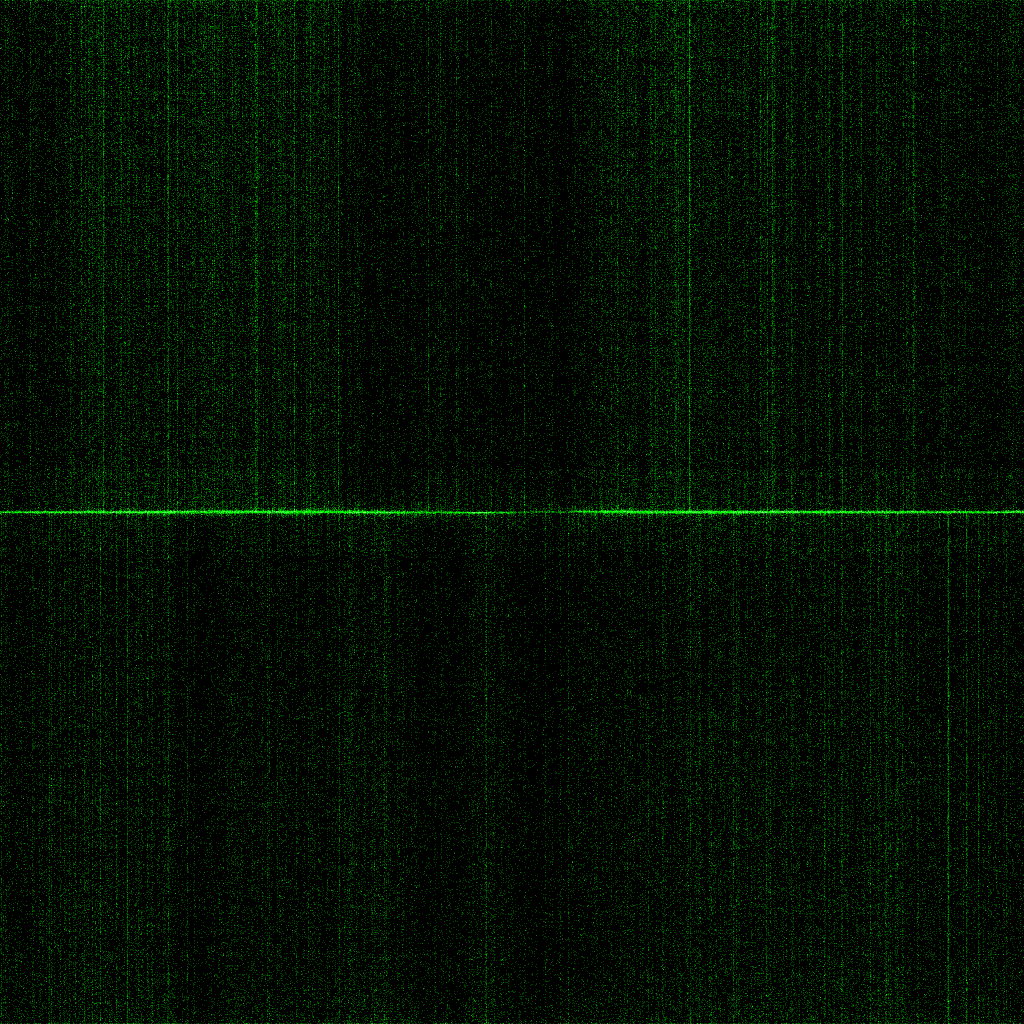
\includegraphics[width=0.6\textwidth]{images/DSNU.png}
    \caption{example of DSNU, 100 frames average with no illumination. The bias fluctuation is seen as regular column patterns.}
    \label{fig:dsnu}
\end{figure}

Noise in digital cameras has a fluctuating behavior, and certain random noises errors can be positive or negative, which means that with a signal of zero and some negative noise, a pixel could have a negative value.
From a software point of view, a negative value can be problematic. To avoid this, a positive offset is added to each pixel's value.

This offset creates a background effect so that, even without light, each pixel has a non-zero value, which is called \textit{bias}.
However, this bias is not constant through each pixel, because of CMOS column-to-column variations. This causes a fluctuation in the bias, which is the \textbf{DSNU}.
Figure \ref{fig:dsnu} shows DSNU on a dark image with no illumination. While illumination does not affect DSNU, temperature and exposure time does (increasing exposure causes sensor to heat).

\section{Challenge-Response Authentication}

Challenge-Response Authentication is a security protocol used to verify the identity of a user by providing a challenge, to which the user must respond correctly.
Often, the challenge would be a random nonce (random number used only once, to avoid replay attacks). The user applies a transformation on the random nonce and sends the response to the verifier.
The CamPUF design uses the DSNU fingerprint as the basis for the challenge-response authentication protocol.
This mechanism has the advantage of having a light communication overhead between the user's device and the verifier, which is useful, since CamPUF is created with low-power devices (mobile devices) in mind.

\begin{figure}[h!]                      % REMEMBER TO REFERENCE THE IMAGE SOURCE
    \centering
    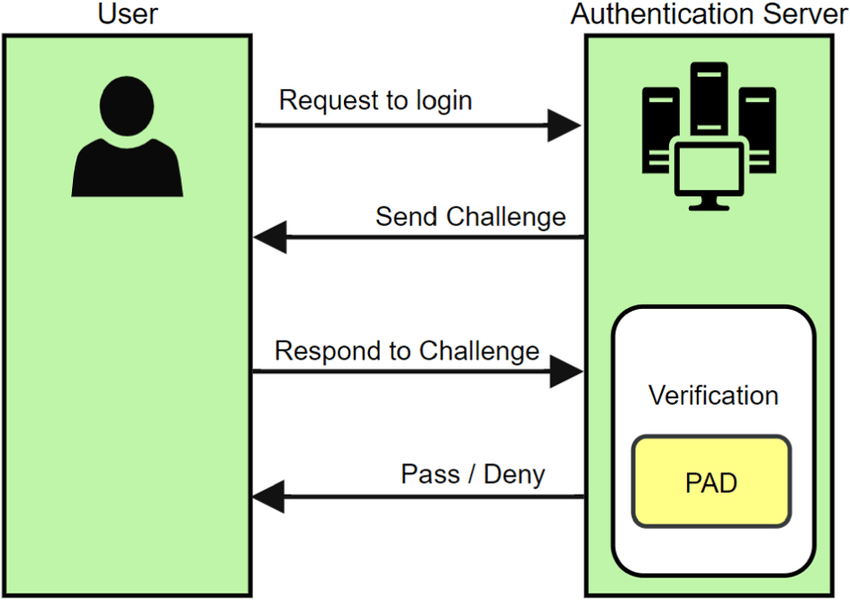
\includegraphics[width=0.6\textwidth]{images/Challenge_Response_Auth.png}
    \caption{Simple schema which shows the Challenge-Response protocol}
    \label{fig:cr_auth}
\end{figure}

The Figure \ref{fig:cr_auth} shows all the protocol steps and parties involved.
